\documentclass[10pt,letterpaper]{article}
\usepackage{amsmath,amssymb}
\usepackage{changepage}
\usepackage[utf8x]{inputenc}
\usepackage{textcomp,marvosym}
\usepackage{cite}
\usepackage{nameref,hyperref}
\usepackage[left]{lineno}
\usepackage{microtype}
\DisableLigatures[f]{encoding = *, family = * }
\usepackage[table]{xcolor}
\usepackage{array}
\usepackage[aboveskip=1pt,labelfont=bf,labelsep=period,justification=raggedright,singlelinecheck=off]{caption}
\renewcommand{\figurename}{Fig}
\bibliographystyle{plos2015}
\makeatletter
\renewcommand{\@biblabel}[1]{\quad#1.}
\makeatother


\usepackage{lastpage,fancyhdr,graphicx}
\usepackage{epstopdf}
\usepackage{orcidlink}
\makeatletter
\renewcommand {\verbatim@font}
{%
  \fontencoding {T2A}%
  \fontfamily
  {\ttdefault}%
  \selectfont
}
\makeatother
\usepackage [russian,english] {babel}

\hypersetup{
  colorlinks   = true,
  urlcolor     = black,
  linkcolor    = black,
  citecolor   = black
}


\begin{document}
\vspace*{0.2in}

\begin{flushleft}
{\Large
\textbf\newline{
Clavis: an open and versatile identification key format
}
}
\newline
\\
Wouter Koch\orcidlink{0000-0001-9025-9486}\textsuperscript{1,2*},
Hallvard Elven\orcidlink{0000-0002-6001-0839}\textsuperscript{3},
Anders G. Finstad\orcidlink{0000-0003-4529-6266}\textsuperscript{1}
\\
\bigskip
\textbf{1} Department of Natural History, Norwegian University of Science and Technology, Trondheim, Norway
\\
\textbf{2} Norwegian Biodiversity Information Centre, Trondheim, Norway
\\
\textbf{3} Natural History Museum, University of Oslo, Oslo, Norway
\\
\bigskip

* wouter.koch@artsdatabanken.no

\end{flushleft}
\section*{
Abstract
}
The skill to recognize and classify taxa requires knowledge that is less and less common in the scientific community. At the same time, it is clear that these skills are needed in biodiversity monitoring for management and conservation, especially when carried out by citizen scientists. Formalizing the required knowledge in digital identification keys is a way of making such knowledge more available for professional and amateur observers of biodiversity. In this paper we describe Clavis, a modern open framework for capturing knowledge required for taxon identification through digital keys, allowing for a level of detail beyond that of any current format. We exemplify each concept using Pokémon as a fictional taxonomic group.
\section*{
Introduction
}
Distinguishing biological taxa from one another is a necessity in biodiversity monitoring. As species are going extinct at an unprecedented rate~\cite{Ceballos2015, Johnson2017}, we need to monitor as much as we can to identify statuses and trends. Meanwhile, research and management is currently facing a ``taxonomic impediment'', where taxonomic knowledge is disappearing from the scientific community~\cite{Engel2021}.

Paradoxically, while taxonomic expertise is becoming scarce, species observations are being reported like never before. The bulk of the observational data currently available originates from citizen science (in which observations are made by non-professional volunteers~\cite{Silvertown2009}). There are, however, large taxonomic biases in the data collected, especially within citizen science. For example, of publicly available data from the Global Biodiversity Information Facility (GBIF, the largest aggregator of biodiversity observations in the world~\cite{GBIFhomepage}), some 67\% of over 2 billion observations pertain to birds~\cite{GBIF_data_taxonomy}. This means that less charismatic species, and species that are more difficult to identify, generally remain severely under-reported~\cite{Troudet2017}. Many such species play important ecological roles or can serve as indicators of broader ecosystem health, but the fact that few observers are able to reliably identify these species leads to their underreporting, obscuring important trends from the view of science and management~\cite{Dobson2020}.

The knowledge needed to identify species resides in large part in the heads of taxonomic experts. This invaluable experience is slowly disappearing however, as newly educated biologists are, to an increasing extent, trained with focus on skills in genetics, data management, and biodiversity informatics rather than traditional taxonomy. This training, and an academic reality of shorter periods with funding and more temporary contracts, gives fewer researchers the opportunity to invest the years of experience needed to become truly knowledgeable with regards to any substantial taxon, as was more commonplace in the past~\cite{Ebach2011}. 
                   
Identification keys are one of the most important tools used by taxonomists to identify taxa, and thus also to share with others the information needed for distinguishing taxa. No taxonomist studying a large taxon in depth can get around identification keys, and keys are often the starting point when trying to learn a new organism group. Identification keys can, however, be quite challenging to use, especially for novel users, and their use often represents a significant barrier for the prospective learner. For this and other reasons, experience with identification keys is something receiving less focus in most current biology curricula. Furthermore, as taxonomic knowledge is becoming increasingly fragmented, existing identification keys in literature are gradually becoming outdated as taxonomies are changing according to new insights.

These issues are exacerbated in the context of citizen science. Whereas prospective taxonomists have a professional incentive to learn to use an identification key, a steep learning curve can quickly put off the more casual citizen scientist. With its unrivaled amounts of data, but also added concerns regarding the reliability of the taxon identifications~\cite{Crall2011,Burgess2017} and the pronounced over-representation of more charismatic taxa~\cite{Callaghan2020,Bayraktarov2019,Boakes2016}, citizen science stands especially much to gain from good identification keys with a low usability threshold.

Digital identification keys can address these challenges in a number of ways. The formalized and machine-readable way in which the data are stored allows for easier revision, as well as multiple options for their display to the end user, tailored to their level of experience. Digital keys allow for the representation of more complex relationships between species' characteristics and identifications inherent to biological complexity. These relationships cannot as easily be represented in a linear form as is used in traditional, paper-based keys. With a suitable interface, they open up the cumulative experience from taxonomic experts to a broader public like citizen scientists, while potentially being more reliable and educational than other identification methods such as automated image recognition. In contrast to paper-based keys, digital keys can also be combined with one another, integrating the information from several separate keys into one seamless user experience. And conversely, a digital key can easily be limited to just a subset of the taxa in it, for instance only taxa belonging to a certain habitat or recorded in a certain geographic range. Another benefit is the option of saving the user input and the key together with the observational data, as a means of transparent identification that can be reviewed at any time in the future for quality control or in the case of new taxonomical insights.

Having a fully open and well-defined, platform-independent format is essential in ensuring that identification keys and the tools needed to display and create these are and remain both interoperable, interpretable across platforms, and freely available to all. A number of digital identification key formats exist~\cite{Dallwitz1980, Lucid}, but these come with a number of caveats in terms of limitations in what they can represent, ease of use, openness, etc. A well-defined format addressing this alleviates the technical burden in capturing taxonomic knowledge for future use.

In this manuscript we document Clavis; an open format for identification keys, aiming to cover the aforementioned requirements in an open and lightweight manner, and serving as an example of a way to store and exchange crucial taxonomic knowledge. Clavis is intended to capture all the requirements of traditional keys while adding the flexibility and complexity possible with digital keys. This means that the format is well suited for representing most, if not all, existing keys, both paper based and digital, as well as for designing new keys. The name Clavis means ``key'' in Latin, and is a recursive acronym for \underline{C}lavis \underline{L}ightweight \underline{A}nd \underline{V}ersatile \underline{I}dentification \underline{S}chema. This article describes the Clavis format itself. Example code handling the business logic of keys described using Clavis will be published separately at a later time. Descriptions of each of Clavis' data types and emerging properties are illustrated here using fictional taxa that are discretely defined and not subject to taxonomic debate or change, while exhibiting the required complexity for a demonstration of the more intricate features of the format. Our fictional creatures of choice for these examples are a selection of Pokémon~\cite{Pokemon_wiki}.

\section*{
Material and methods
}
Identification keys exist in many forms, but all are built on the same basic principle. The user is asked a number of questions about the entity being identified, and by answering these questions, more and more taxa are excluded from consideration until (ideally) only one taxon remains, which is the result of the identification process.

Traditional single access keys consist of a decision tree with a single fixed path from beginning to end for each possible outcome. On choosing an answer from the alternatives for each of the questions, one is directed to the next question to be answered, until one ends up with a result taxon. Such keys can be either dichotomous, meaning that each question always has only two alternatives, leading to a bifurcating decision tree, or they can be multichotomous, meaning that each question may have more than two alternatives. One upside of single access keys is that they are easy to represent on paper. A drawback is that a user has to go through all questions in a specific order, having one and only one question to answer at any given time. This means that one cannot use only part of the key for a subset of taxa, nor easily go back and redo a question. Also, if a question cannot be answered, there is no way to proceed.

An alternative approach is the multiple access key. Such keys are typically stored as matrices where taxa and questions (characters) are stored as rows and columns in a tabular format, with cell values linking the taxa to their characters. Each character may have two or more possible answers (states), or be defined as a numerical value or range of values. This allows for a selection of taxa to be made that one wishes to distinguish between, rather than having to traverse the entire key. In a fully populated matrix key, every character is assigned a value (i.e. is scored) for every taxon. The user then has access to all the questions/characters at once and is not required to answer them in any particular order. Choosing any alternative for any of the questions will exclude from consideration all those taxa that are not compatible with that alternative, bringing the user a step closer to the answer. The upside of this approach is that the user has several paths to the answer, and can choose to avoid questions that are difficult or impossible to answer. The downside is that the number of choices can easily be overwhelming, and it is generally left to the user to try to choose the best path. Also, in real life situations it is very rare to find a set of characters that are both possible to score in a meaningful way for all the taxa in the key, and sufficient for distinguishing between them. More often, some characters will be possible to score for all taxa, whereas others may be essential for distinguishing certain taxa in the key, yet be totally inapplicable to others.

To address this, a matrix can also be made to be sparse, meaning that not all characters are scored for all taxa. The interface can then display only those characters that have been scored for all the taxa under consideration. As taxa are being excluded by the user’s choices, further characters that are scored for all the remaining taxa will become available. With this approach, it is possible to make a matrix key that behaves equivalently to a single access key. But the key can also be made to contain several distinguishing characters for any set of taxa, so that the user has more than one choice at each step and is thus not restricted by having to answer only one question at a time in a specific order.

The sparse matrix approach is more powerful than both the single access and the full matrix approach, in that both of the latter approaches are subsets of what the sparse matrix can represent. Still, there is much information one would ideally like to store about taxa, characters, and the relationships between the two, which cannot be easily represented in a tabular format. For instance, the tabular format is not well suited for dealing with polymorphism in a straightforward way, i.e. the situation where a taxon can have more than one possible value for a given character. Also, it may often be desirable to treat taxa hierarchically rather than as a simple list of equally ranked entities, something which is difficult to do in the matrix format. Thus, representing taxonomic knowledge in this tabular format restricts the complexity of the information that can be stored.

The method of storing and exchanging taxonomic knowledge described here, is developed as a non-tabular multiple access key. The core of any Clavis key is a collection of statements. A statement links a taxon to a character, and specifies the state or numerical value the taxon has for that character (see Fig.~\ref{fig1}). E.g. the color (character) of species x (taxon) is red (state), or the length in mm (character) of genus x (taxon) is 4-11 (numerical range).




\begin{figure}[!h]
  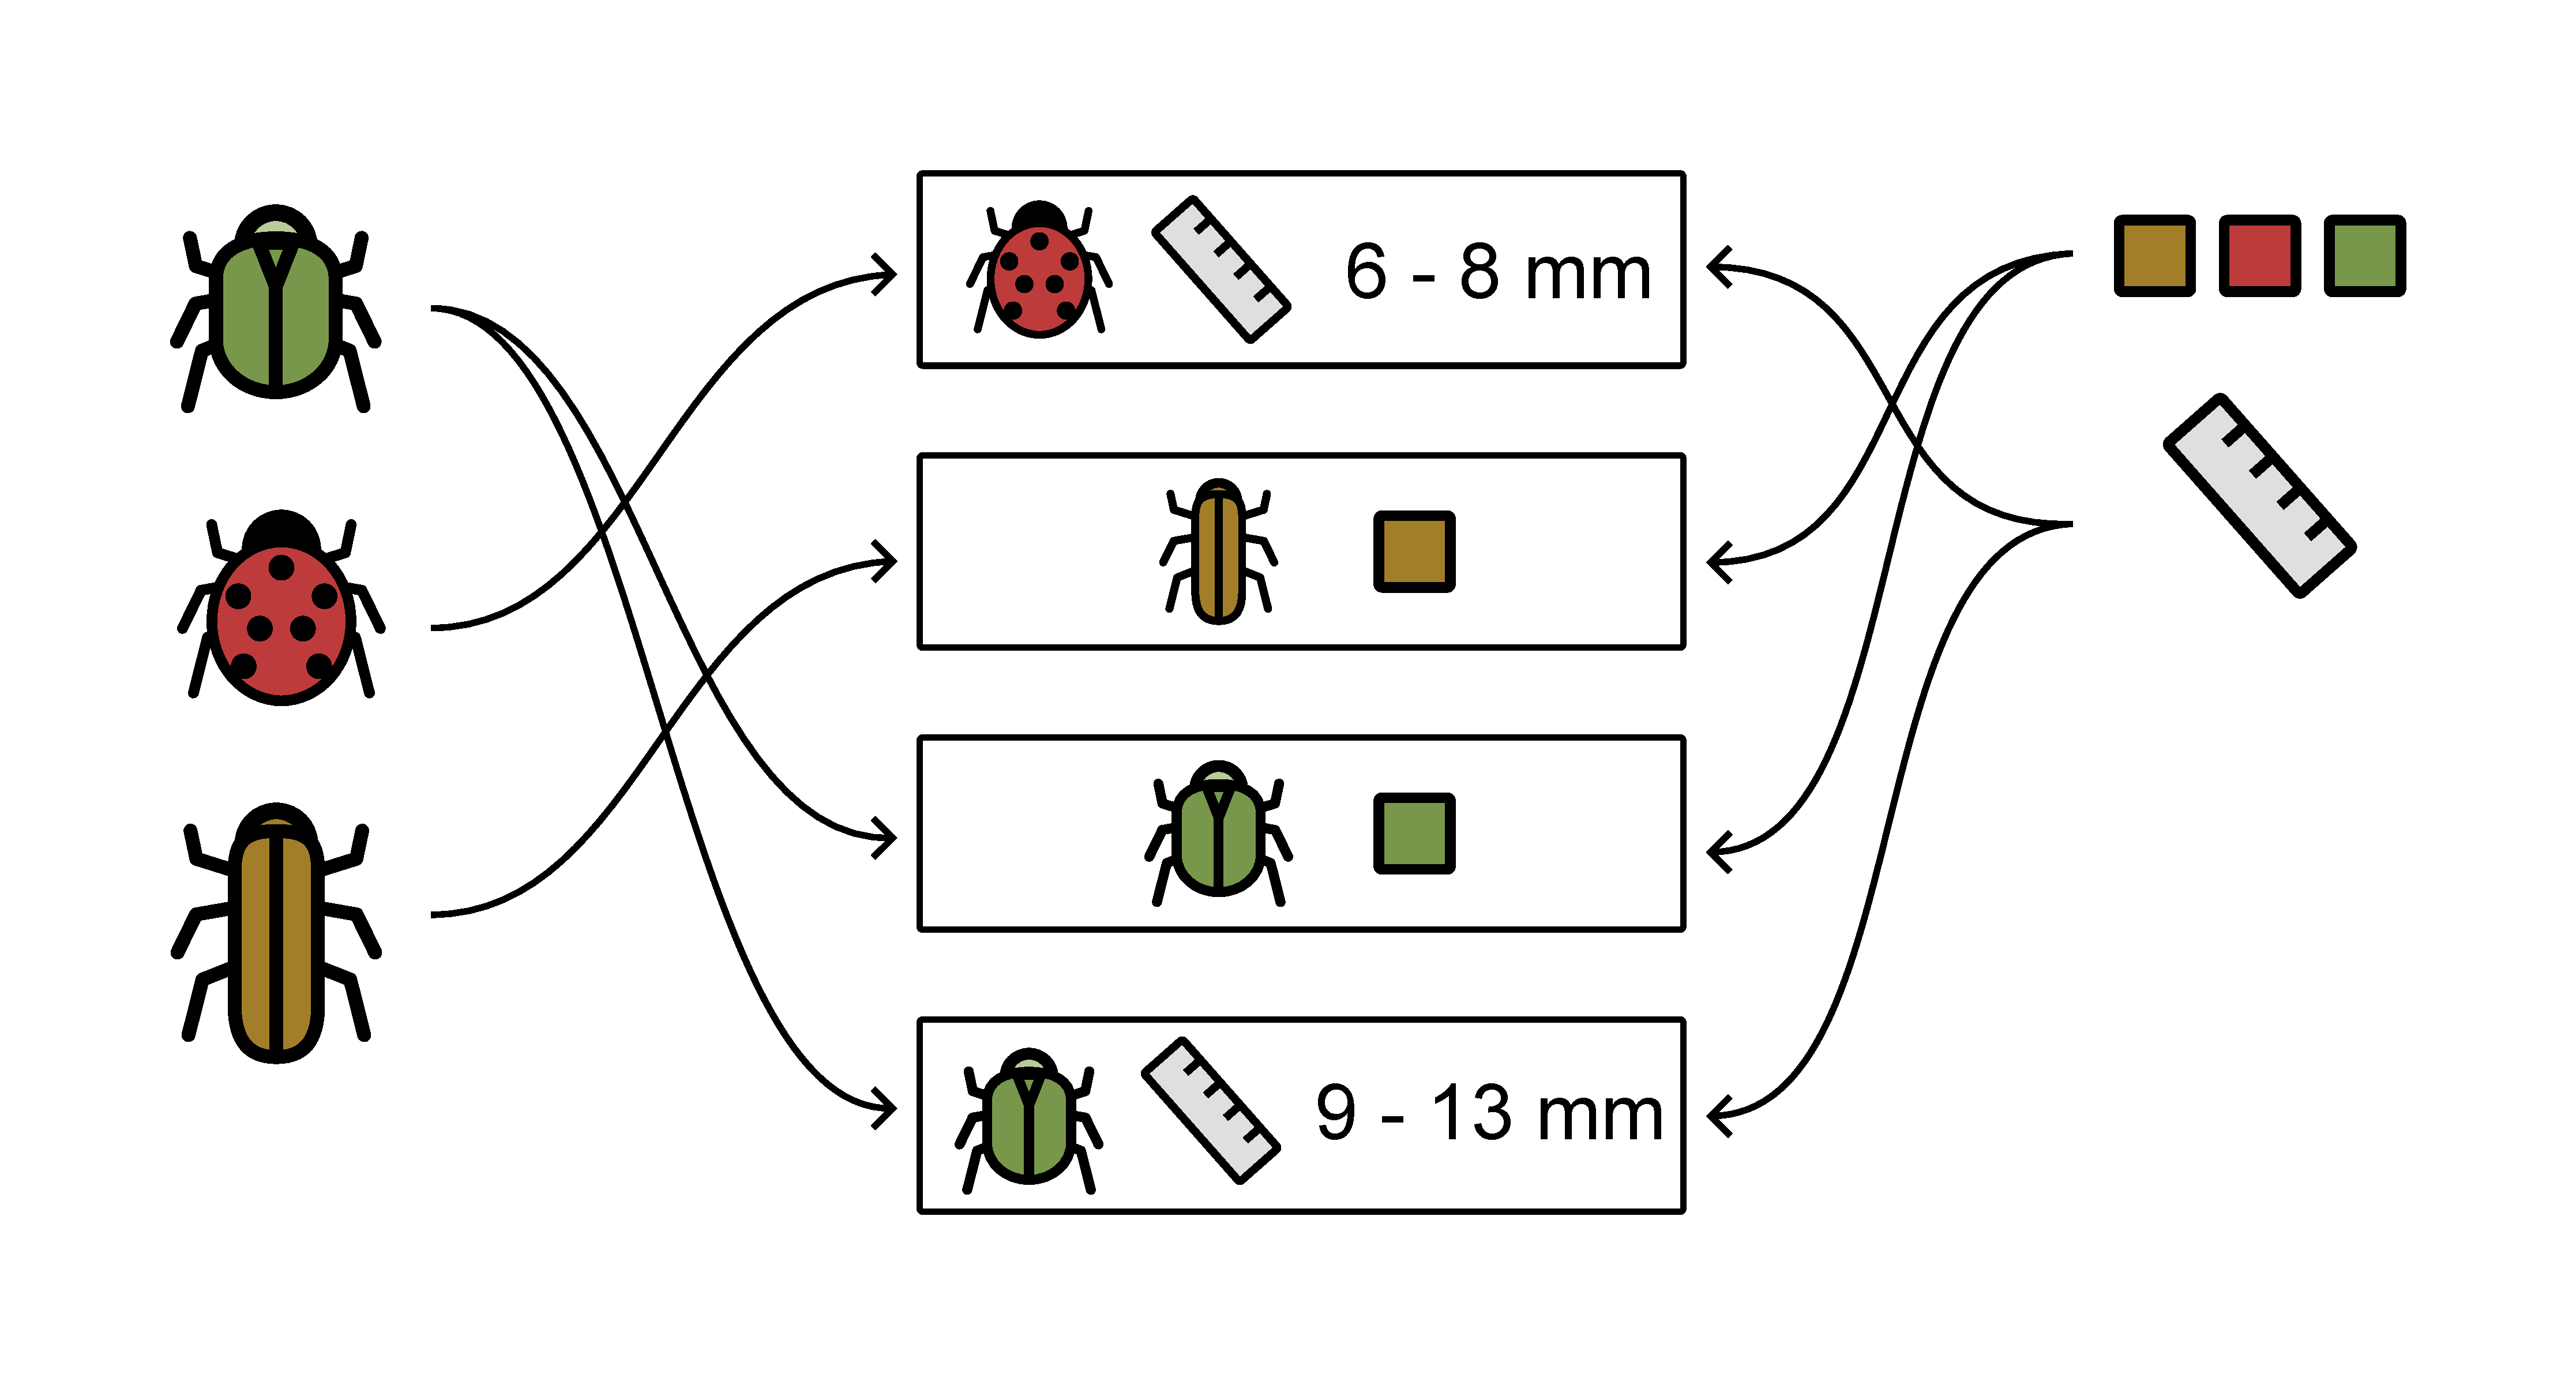
\includegraphics[width=\textwidth]{Images/Fig1}
  \caption{{\bf The core concepts of any Clavis key.}
  \underline{Taxa} (left) and \underline{characters} (right) are connected through \underline{statements} (center). Each statement refers to one taxon and one character, linking the two by a value, usually one of the possible \underline{states} of the character, or a numerical value.}
  \label{fig1}
\end{figure}




Additional information can be linked to taxa, characters, states and statements in a number of ways, capturing knowledge and relationships that cannot be represented in a tabular form in a practical way. Such information includes media elements, textual descriptions, and contextual information such as geographic scope. The Clavis format incorporates all the possibilities of the previously described approaches, so that any single access or matrix key can be transcribed to it.

Clavis compliant keys are written in JSON (JavaScript Object Notation)~\cite{JSON}, which has become the \textit{de facto} standard for data exchange over the internet, as it is an open, flexible format with widespread use and support within all modern programming languages. Clavis itself is a JSON-schema~\cite{JSON_schema}, a formal definition of the structure and content of a valid Clavis JSON file. JSON-schemas are machine readable and can be used to automatically validate the compliance of a JSON file, highlighting any issues that need to be solved. While possible, it is generally not practical to manually write the JSON of a Clavis-compliant key. In order to facilitate key creation and editing, one would generally provide taxonomists with a key editing interface that lets them easily record their knowledge, and let the key editor generate the JSON. The latest version of Clavis can be found at \url{https://github.com/Artsdatabanken/Clavis}.

\subsection*{
Implementation
}
As an exchange and storage format, Clavis does not dictate how it is to be implemented. Different interfaces can implement it differently, depending on the purpose of the interface and the user group. To this end, interfaces serving to edit or display may disregard certain non-essential functionality supported by Clavis. One could for example create a key editor not supporting media files or multilingualism. Other aspects of the format are crucial however, and require support and unambiguous interpretation.

Identification is a matter of excluding taxa, and is done by letting the user select a state or numerical value for characters. Each time the user provides a new fact in this way, all taxa with conflicting statements are excluded (see Fig.~\ref{fig2}). The user can also be given the option to exclude a state rather than affirm one if there are more than two states to choose from. Characters that have not been answered but only have a single possible answer remaining for all remaining taxa can be hidden.


\begin{figure}[!h]
  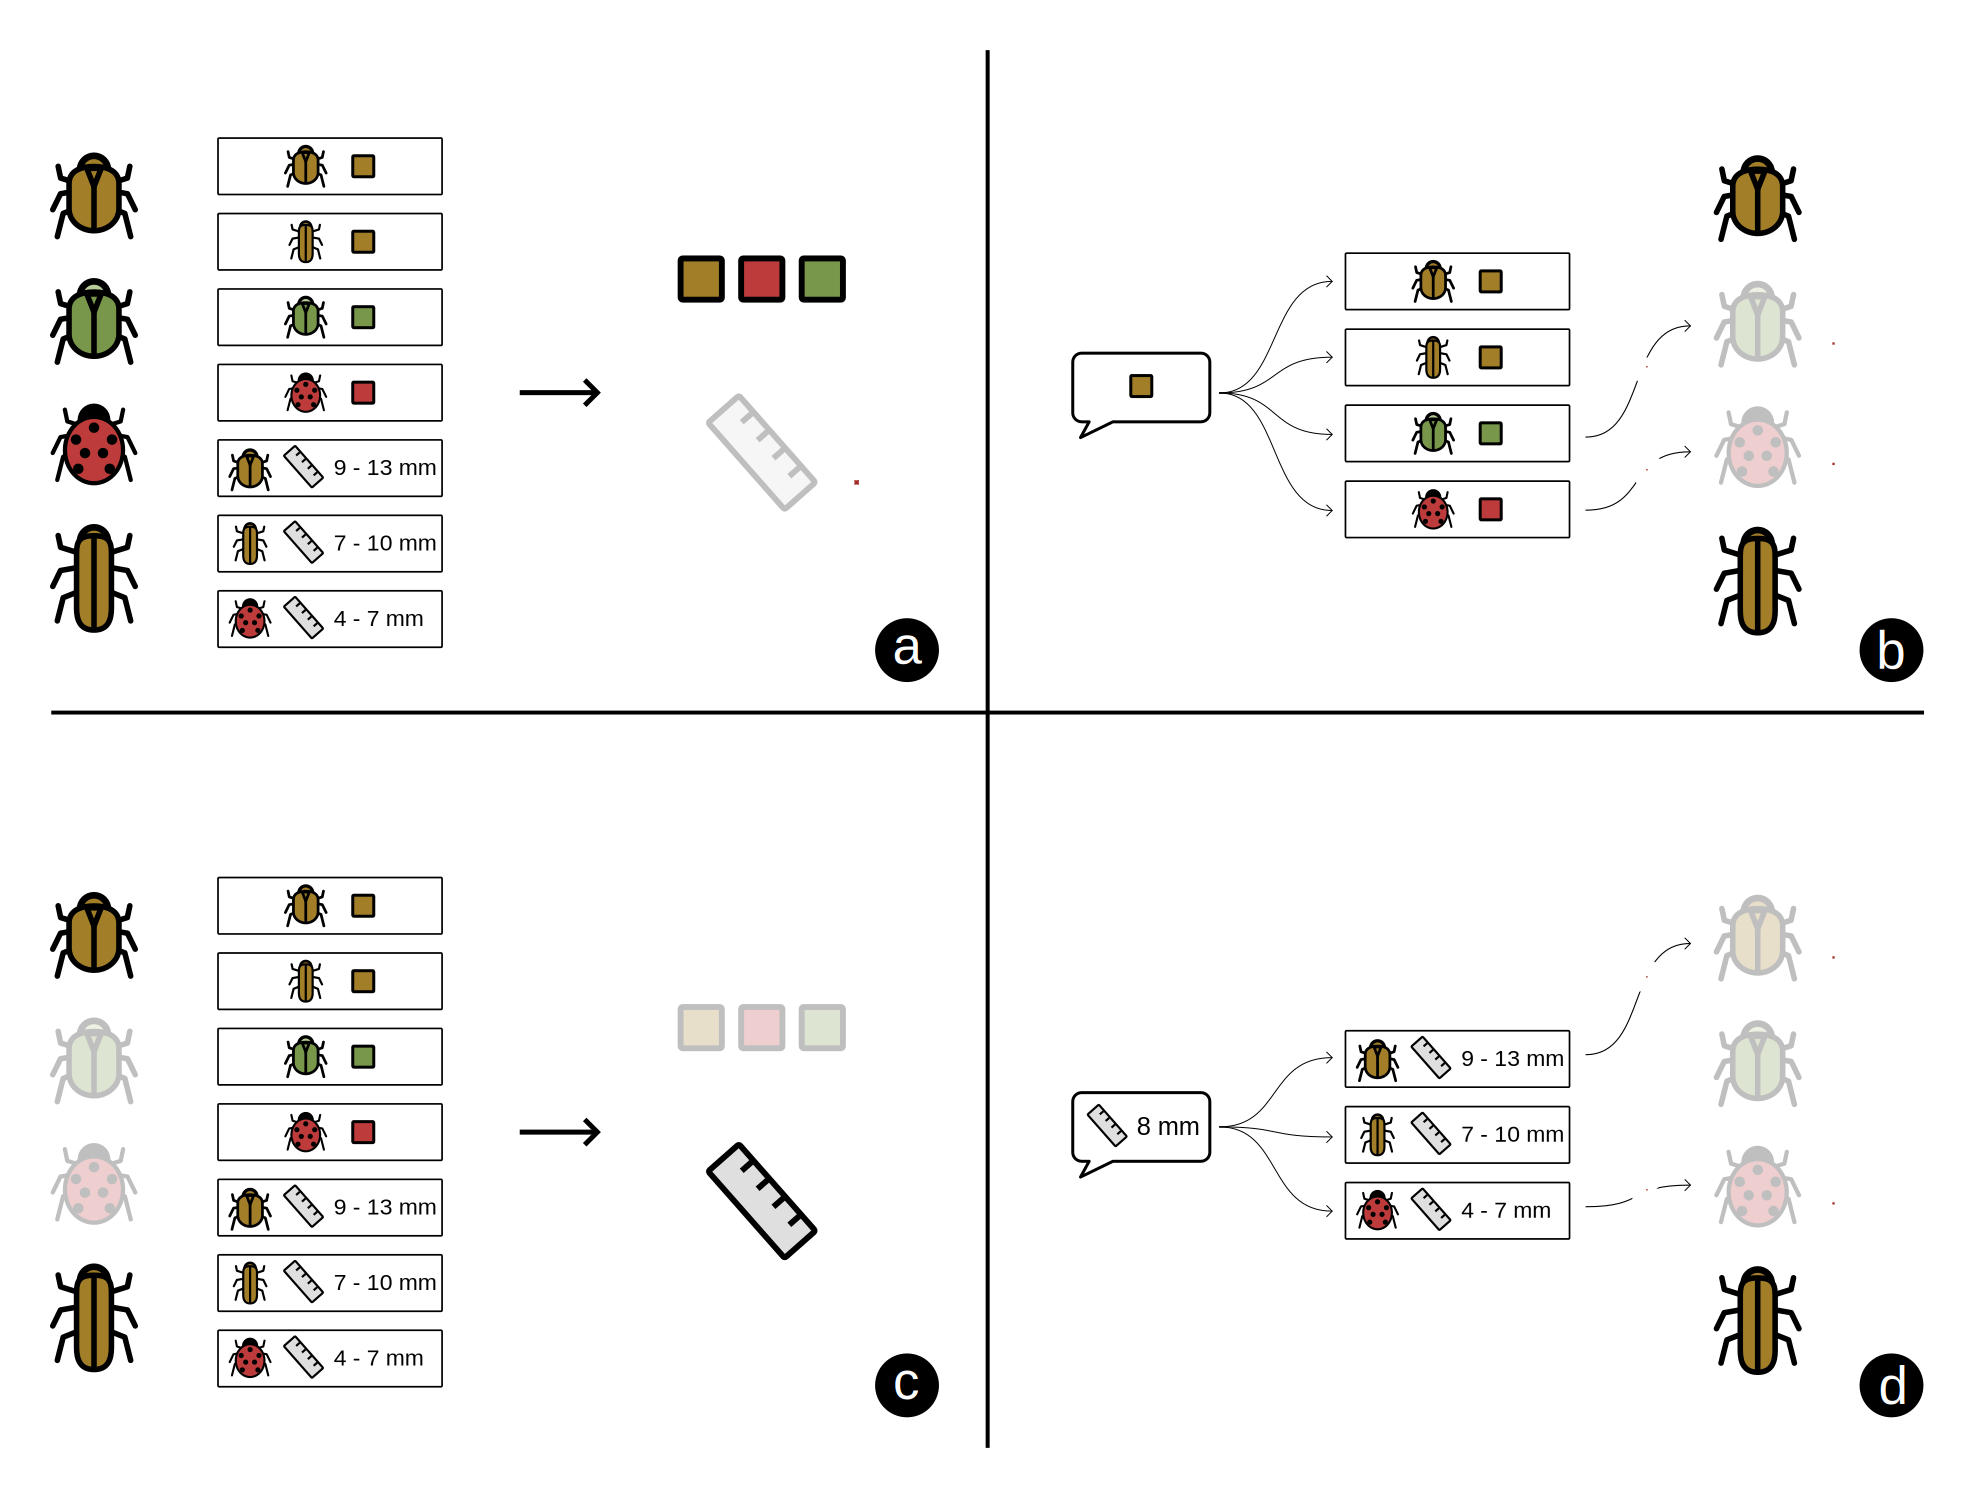
\includegraphics[width=\textwidth]{Images/Fig2}
  \caption{{\bf The identification of a specimen.}
  When considering all taxa, the character about size is not relevant, as one of the taxa has no statement for size, so only the character about colors is relevant (a). The user gives an input, which is compared to the related statements, upon which 2 taxa are eliminated (b). Considering the now remaining taxa, the character about size has become relevant (c). The user gives another input, and based on the related statements, one additional taxon is eliminated, leaving one result (d).
  }
  \label{fig2}
 \end{figure}

Whenever taxa are excluded, characters that were previously hidden may now have become relevant if all the remaining taxa have a statement pertaining to it, as illustrated in Fig.~\ref{fig2}. It is important to check for states that, while not having been answered directly by the user, can be deduced from the statements related to the remaining taxa: if all the remaining taxa are known not to have a certain state, that state can be disabled. In such cases, the state still needs to be visible to the user as it provides context to the remaining options, but it should not be possible for the user to select it. In all cases, only characters that are linked by statements to \underline{all} the currently non-excluded taxa should be shown to the user.

Things become more complicated when allowing the user to undo previous answers. Undoing an answer might render a character that was subsequently answered irrelevant again. To avoid answers to this now irrelevant character from eliminating taxa as possibilities, an implementation needs to be able to remove or ignore such answers on characters that were rendered irrelevant.

The provided schema ensures that a key adheres to the Clavis format in a technical sense, but it does not ensure that any compliant key is logically complete and consistent. One can make a valid key that contradicts itself or that does not contain sufficient information to reliably distinguish between certain taxa. It is advisable to implement checks for this in any key-editor, and when keys by third parties are to be displayed, to also ensure such cases are handled by the end-user interface.

To illustrate the features supported by the Clavis format, we here describe features and give some example uses. The examples relate to fictional creatures that are not subject to taxonomic debate or change. For this we chose Pokémon as they appear in the mobile game Pokémon Go, as these are clearly defined, yet exhibit the complexity required to demonstrate the various features of the format. Keys for natural taxa would rarely use as much of the possible functionality as we demonstrate here in a single key. The key is valid in accordance with the JSON-schema, but it does not contain all the information needed to distinguish between all of the Pokémon mentioned in it. We also provide an example of a non-artificial key that does identify all taxa in it, but without aiming to demonstrate all possible features that Clavis supports. This key covers all species of titmice in Norway and can be found in the supplementary material.

\section*{
Results
}
The main components of the Clavis JSON-schema are the taxa that the key is designed to distinguish between, the characters describing relevant properties, and statements connecting taxa to characters through states or numerical values. Additionally, the schema defines a number of metadata fields, as well as custom data types, that can be referred to in various places in the key, such as when referring to a person as a creator of a picture or linking a picture to a taxon.

\subsection*{
Format overview
}
An overview of the elements in an identification key defined by Clavis. Elements with an asterisk (*) are mandatory.

\subsubsection*{
Key metadata
}
\begin{itemize}
\item[\textbf{Title*}]
The name of the key
\item[\textbf{Schema*}]
The url of the version of Clavis that the key adheres to
\item[\textbf{Media}]
A media element for the key, such as a logo or icon
\item[\textbf{Description}]
A short, extended, and/or external description of the key
\item[\textbf{Audience}]
A description of the intended audience
\item[\textbf{Source}]
Name and/or link to the source the key is based upon
\item[\textbf{Geography}]
Polygon of where the key is valid
\item[\textbf{Roles}]
Primary contact, creators*, contributors, publishers of the key, as references to persons and/or organizations
\item[\textbf{License*}]
An url to the license text the key is licensed under
\item[\textbf{Language*}]
The language(s) the key supports. Texts for multiple languages in other key objects are in the order defined here
\item[\textbf{Dates*}]
The dates the key was created and last modified (the version)
\item[\textbf{Identifier*}]
An id for the key, that remains stable over versions
\item[\textbf{Url}]
Where the key is hosted, so that new versions can be retrieved
\end{itemize}
\subsubsection*{
Key content
}
\begin{itemize}
\item[\textbf{Taxa}]
A flat or hierarchical list of taxa the key is able to distinguish between. The goal of the interface is to eliminate all but one taxon.
\item[\textbf{Characters}]
A list of characters used to distinguish between taxa. These are the questions that are to be presented to the user. A character can be categorical or numerical. When categorical, it has a list of states that are the relevant alternatives for this character.
\item[\textbf{Statements}]
Elements connecting a taxon to a character state. This is the core knowledge captured by the key: which taxa have which states or numerical values for which characters, thus distinguishing them from one another.
\end{itemize}
\subsubsection*{
Data types
}
\begin{itemize}
\item[\textbf{Person}]
The name*, contacts, media elements, and affiliations of a person.
\item[\textbf{Organization}]
The name*, contacts, and media elements of an organization.
\item[\textbf{Taxon}]
The scientific name*, author, vernacular name, media elements, rank of a taxon. Info on whether it is a sub-taxonomic unit, and if it serves as an end-point or not. It can have a set of children, which are the underlying taxa. An external reference can define where info is to be retrieved from. It may have a geographic distribution as an object or external service, to assess where it occurs. A follow-up key as a url or external service reference can provide info on where a more detailed identification can be done.
\item[\textbf{Character}]
The name* and states* describing a property a taxon can have. It can have media elements and descriptions clarifying the character, and a user requirement. A logical premise can specify what other user input has to be given before the character may be presented. A character can be of the types ``exclusive'' (default, multiple choice where options exclude one another), ``non-exclusive'' (multiple choice with multiple answers possible), and ``numerical'' (the answer is a number). A character has states defining the possible answers.
\item[\textbf{State}]
A possible answer for a character. Has either a title if the character type is non-numerical, or a min, max, step size and unit if it is numerical. It can have multiple media elements and descriptions clarifying the state. 
\item[\textbf{Statement}]
A connection between a taxon and a character through a value (either a state or a numerical range). It defines how frequently and in which context the taxon has this value for that character. A statement can have any frequency from 0 to 1, to indicate that the taxon always (1), never (0) or in some cases (values between 0 and 1) has this value for the character. A numerical value can be a single value or a range. Statements can contain references to a geographic distribution (or a service providing one), defining where this statement is valid. Media elements and descriptions can be added describing the relationship between the taxon and character in more detail.
\item[\textbf{User requirement}]
A user requirement can have a title, media elements and descriptions describing certain skills, equipment or other requirements needed to evaluate a character. It can also have a warning text to alert the user of these requirements. It can be used to guide a user where necessary, or help the user decide whether to skip more challenging characters.
\item[\textbf{External service}]
A reference to an external service and its documentation. The creator of an interface can then choose to implement this external service so that e.g. taxon names are retrieved from an up to date repository by the provided stable identifier.
\item[\textbf{Media element}]
A media element contains the data needed to display multimedia files. It can refer to different versions for different languages, and can have different versions for different media dimensions. It contains the required metadata such as width and height (images and video), length (sound and video), as well as creators, contributors, publishers and a license. Files can be urls to where the correct version of the file is to be found, or directly contain a base64 or svg encoded file. It supports external services to retrieve such information from elsewhere.


\end{itemize}

\subsection*{
Statements
}

The core element of any key is the statement. It defines a property of a taxon, separating it from other taxa with conflicting statements. In JSON (object) notation, a single statement takes the following form, in this case stating that Pikachu is an electric type Pokémon.

\begin{verbatim}
{
   "id": "statement:pikachu_is_electric",
   "taxonId": "taxon:pokemon_025",
   "characterId": "type_of_pokemon",
   "value": "state:pokemon_type_electric",
   "frequency": 1
}

\end{verbatim}

While all core concepts are described with examples, not every combination of concepts are exemplified here. So while both multilingualism and descriptions are demonstrated, there is no example of multilingual descriptions. Such features do follow the same logic as the examples provided, and are all specified in the JSON schema.

\subsection*{
Key metadata
}
Very few parameters are required on the top level of the key. Apart from the content of the key (taxa, characters and statements linking the two), a key is expected to refer to the version of the schema with which it complies, a title, language, license, a creator, the date at which it was last modified and an identifier that is to be kept stable across versions. As the creator is expected to be a reference to a person entity, one also needs to define at least one person.

\textit{\textbf{Example}: See lines 2 - 10 in the \nameref{S2_Appendix} for the corresponding JSON.}

\subsection*{
Taxa
}
Eliminating all but one taxon is the goal of the user, and taxa are the units that all characteristics are connected to. Taxa can be provided as a simple (flat) list, but they can also be structured hierarchically, commonly, but not necessarily, adhering to their phylogeny. Statements can in such a hierarchy be connected to higher taxa, reducing a lot of the repetition of traits shared within a taxon that one would get in a simple list of taxa. If a statement is tied to a higher taxon in the hierarchy, it is implied that all the underlying taxa share the same statement.

In addition to biological taxonomic units, one can also define sub-groups within a taxon. Examples can be different sexes, morphs, or species complexes. Contrary to regular taxa, such subdivisions of taxa are not standalone taxonomic units. As such, they do not have their own scientific name but rather a label that adds specificity to their parent taxon. For example, the label of a sub-group specifying the sex of Pikachu would simply be ``\Female'' rather than ``Pikachu \Female'' as it already relates to the parent ``Pikachu''. For a default form of a taxon, the label can be an empty string.

The goal of the key is to provide a way to eliminate all but one taxon; the end point of the key.  The key should stop asking questions once the user has narrowed down the possible outcomes to a single end point. In a flat list of taxa, every taxon in the list will normally be an end point. In a hierarchical list, the lowermost taxa in the hierarchy will be the end points by default. This can be overridden, however, by explicitly tagging a taxon higher up the tree as an end point. Then, information on lower taxa may be displayed when identified while using the key, but no additional questions are asked once the end point has been determined. This can be used, for instance, to display an image of the relevant sub-group for a taxon, so that the taxon images reflect the input from the user.

\textit{\textbf{Example}: Pichu, Pikachu and Raichu are all species within the Pikachuidae. They each have a default and a ``Shiny'' morph, which is to be determined. The default Pikachu morph also has a subdivision into the sexes, but as the morph is tagged as an endpoint the user will not be asked further questions to determine these once the morph has been determined. See lines 25 - 94 in the \nameref{S2_Appendix} for the corresponding JSON, and Fig.~\ref{fig3} for a graphical representation.}


\begin{figure}[!h]
  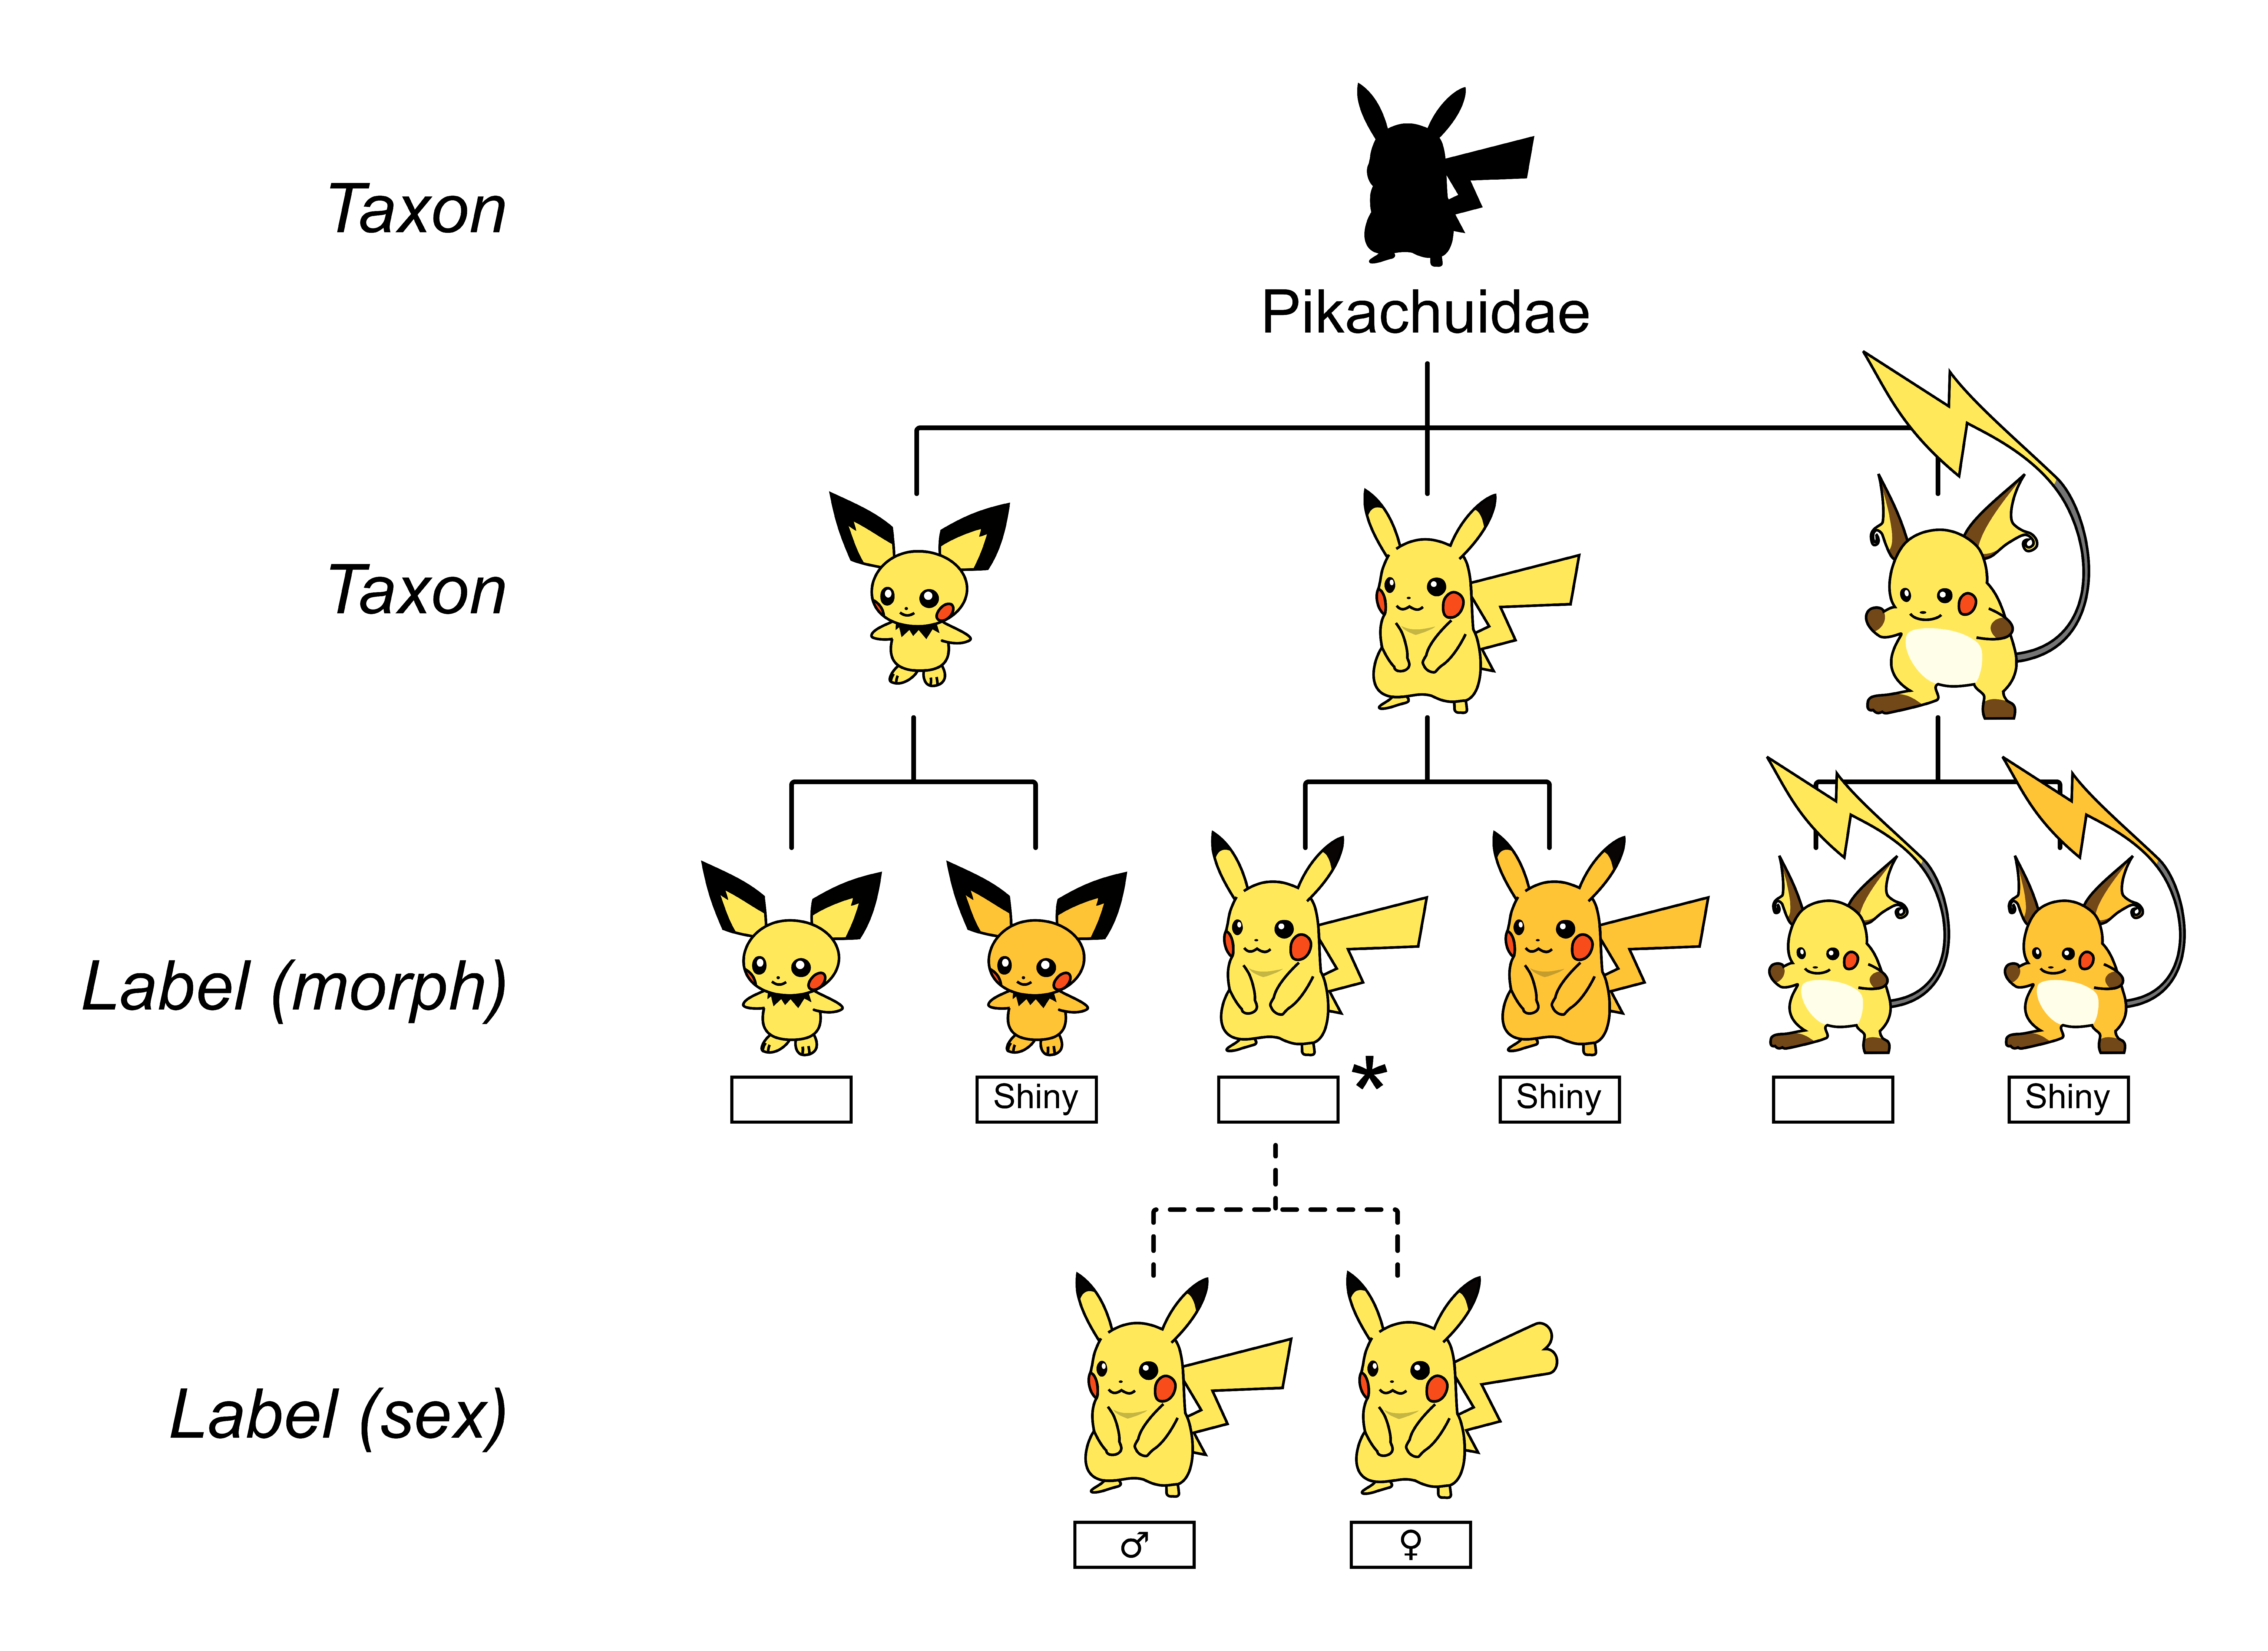
\includegraphics[width=\textwidth]{Images/Fig3}
  \caption{\textit{\textbf{A taxon tree of the Pikachu-line}:
Taxa tagged as endpoint are indicated with an asterisk (*). This key continues until the correct morph (``Shiny'' or default) is known, while differences in the sexes are optional and will not be asked about once the correct Pokémon and morph have been determined.
  }}
  \label{fig3}
\end{figure}
\subsection*{
Characters, statements and frequencies
}
One of the possible values for a statement (the relationship between a taxon and a character) is the id of a state. This statement also may have a frequency: the proportion of cases where individuals of this taxon have this state for this character. It can be set to 0 or 1 or any value in between.

In the default setting, the states of a character are interpreted as being mutually exclusive. If there is a character with states ``blue'' and ``red'', a specimen may be either blue or red, but not both at the same time. This means that a taxon that is noted as always being blue is known never to be red, and vice versa. This default behavior can be overridden, however, by defining the character as non-exclusive.

\textit{\textbf{Example}: Pikachu is always an electric type. See lines 264 - 270 in the \nameref{S2_Appendix} for the corresponding JSON.}

\textit{\textbf{Example}: Pikachu is never blue. Note that it is not inferred that Pikachus therefore are red. See lines 271 - 277 in the \nameref{S2_Appendix} for the corresponding JSON.}

\textit{\textbf{Example}: Pikachu has a double-lobed tail in 50\% of the cases. See lines 278 - 291 in the \nameref{S2_Appendix} for the corresponding JSON.}
\subsection*{
Multilingualism
}
Rather than referring to a single language by its ISO 639-1 code, one can make a key multilingual by specifying an array of language codes that are supported. When doing so, strings within the key that differ between languages have to be given as localizedStrings, objects containing a version of each of the supported languages. To support different script types, also strings like people's names support localizedStrings.

Not only strings can have different versions for different languages. Links to external online resources can refer to separate language versions (localizedUrls), and images (e.g. containing text) can have different versions for different languages too (localizedMediaElements).

\textit{\textbf{Example}: A creator name requiring different transcriptions within a multilingual English/Ukrainian key}
\begin{verbatim}
"language": ["en", "uk"],
"creator": "person:wouterkoch",
"persons": [
   {
     "id": "person:wouterkoch",
     "name": {
       "en": "Wouter Koch",
       "uk": "Ваутер Кох"
     }
   }
]

\end{verbatim}

\textit{\textbf{Example}: A creator name that needs no translation, and a character that does, within a multilingual English/Dutch key}

\begin{verbatim}
"language": ["en", "nl"],
"creator": "person:wouterkoch",
"persons": [
   {
     "id": "person:wouterkoch",
     "name": "Wouter Koch"
   }
],
"characters": [
   {
     "id": "character:eye_color",
     "title": {
        "en": "Color of the eyes",
        "nl": "Kleur van de ogen"
     },
     "states": [
       {
         "id": "state:blue_eyes",
         "title": {"en": "Blue", "nl": "Blauw"}
       },
       {
         "id": "state:red_eyes",
         "title": {"en": "Red", "nl": "Rood"}
       }
     ]
   }
]

\end{verbatim}

\textit{\textbf{Example}: An organization with names and urls within a multilingual Norwegian/English key}

\begin{verbatim}
"language": ["no", "en"],
"publisher": "organization:ntnu",
"organizations": [
   {
     "id": "organization:ntnu",
     "name": {
       "no": "Norges teknisk-naturvitenskapelige universitet",
       "en": "Norwegian University of Science and Technology"
     },
     "url": {
       "no": "https://www.ntnu.no",
       "en": "https://www.ntnu.edu"
     }
   }
]

\end{verbatim}
\subsection*{
Persons and organizations
}
Persons and organizations can have multiple roles in different contexts. A person can be a contact person for a key, and one or more persons can be creators or contributors to a key. Persons can also be creators or contributors to media files. A person can have one or more organizations as their affiliation, and organizations can have a person as a primary contact. An organization can be the publisher of a key or media file, and the primary contact for a key can also be an organization instead of a person.

Persons and institutions can have resources such as urls and mediaFiles connected to them, e.g. institutional websites, portraits and logos.
\textit{\textbf{Example}: Definition of a person and an organization. See lines 11 - 23 in the \nameref{S2_Appendix} for the corresponding JSON.}
\subsection*{
Geographic and taxonomic scope
}
Regions can be defined using a GeoJSON MultiPolygon. On the top level, ``geography'' can be specified to indicate what geographic region the key covers. One can also define a geography at the taxon or statement level, to provide information on where the taxon occurs, and in which region a taxon has that particular relationship to a character. Within a region specified as the geography of a statement, the statement with a geography takes precedence over the conflicting statement without a stated geography.

\textit{\textbf{Example}: Kangaskhan only occurs in Australia. See lines 95 - 146 in the \nameref{S2_Appendix} for the corresponding JSON.}

\textit{\textbf{Example}: The rain form of Castform has a higher frequency in the rainy city of Bergen. See lines 302 - 347 in the \nameref{S2_Appendix} for the corresponding JSON.}
\subsection*{
Logical premises
}
Not all characters make sense in every context, and it is sometimes desirable to be able to specify conditions that must be met before a character is shown to the user. Such a condition may be that the user has given a certain answer to some other character in the key first. To this end, characters can have a logical premise, a JavaScript notation string referring to which facts have to be established for it to be relevant. Logical premises can also relate several facts combined, including numerical values, and can be built using unary and binary operators in JavaScript notation.

While seldomly required for a key to work in general, logical premises can be used to ease the identification process. If characters are scored only for those taxa for which they are relevant for distinguishing, this in itself will normally ensure that the characters stay hidden from the user until they are relevant. However, a situation may arise if some of the taxa in the key are polymorphic, i.e. if they either may or may not have a certain character. In this situation, a character can become visible to the user because all the remaining taxa \textit{can} have it, which will likely cause confusion if the actual target specimen does \textit{not} have it, or it is not observable. By introducing a logical premise such a character may be hidden unless the user has indicated that the specimen does in fact have the character.

\textit{\textbf{Example}: Pikachu caught during special events have hats, in contrast to those caught outside of such events. Other Pokémon (e.g. Honchkrow) always have hats. This allows for the characteristics of the hat to be used in identification, but only when one is not only left solely with Pokémon that can have hats, but when it has been established that the target Pokémon in fact is wearing one. See lines 220 - 248 in the \nameref{S2_Appendix} for the corresponding JSON.}
\subsection*{
Numerical values
}
The possible values that a character can have can take the form of a set of discrete states, such as ``present''/``absent'', or ``red''/``blue''. Others may however come in the form of numerical values, such as counts or measurements. In a key this can be implemented with a character of the type ``numerical''. One can specify the range (min and max) the character can have, the step size and the unit. Statements specifying values for such characters to any taxon can have a range, or a single value. In cases where more advanced metrics are needed, such as a probability function over the numerical values for use in Bayesian analysis, this can be implemented through a call to an external service (see below).

\textit{\textbf{Example}: The weight of a Pokémon varies, both between individuals within a species and between species. To distinguish Pokémon based on their weight, this is added as a numerical character, where weights can be specified in whole kg within a given range. A statement can then be included to register the possible weight range of a given taxon. See lines 249 - 261 (character) and lines 292 - 301 (statement) in the \nameref{S2_Appendix} for the corresponding JSON.}
\subsection*{
External services
}
Various units in a key may be subject to changes that are ideally managed outside the key, in designated centralized systems. Taxon names can change, as can urls to supplemental information, media files, geographic ranges etc. Other parameters, such as the probability distribution of a numerical character for a given taxon, may be too detailed for direct inclusion in a key. It is best practice to not duplicate such resources, but to harvest these via an API or other service interface. To facilitate this, Clavis allows the specification of external services, where documentation for use of the service can be linked. Various units in the key, such as taxa, can refer to such external services through one or more externalResources, connecting the service and the relevant external id to the taxon at hand.

External services should not contain information critical to the workings of the key, as not every implementation can be expected to contain the necessary code to retrieve the information the service provides. External services are however useful for features steering presentation, and can provide complex information that depends on various user inputs and other contextual information. To sort taxa by probability, for example, an external service may provide probability scores for taxa based on the geographic location of the user, the season, and properties like coloration and size of the specimen. An interface that does not implement calling this service will simply not sort the taxa, but still be fully functional.

\textit{\textbf{Example}: To allow for features such as the retrieval of the name of a Pokémon in different languages, one can use a Wikidata query. See lines 435 - 439 (service) and lines 47 - 50 (externalResource) in the \nameref{S2_Appendix} for the corresponding JSON.}

\textit{\textbf{Example}: A hypothetical API returns the probability for a provided taxon, given its location and size. See lines 440 - 446 in the \nameref{S2_Appendix} for the corresponding JSON.}
\subsection*{
Required expertise
}
Some characters are harder to evaluate than others, and may even require special equipment. To warn and assist users, a key can contain userRequirements, describing such required skills. These requirements can be connected to characters so that the user might filter out characters requiring skills or equipment they do not have, be presented with additional info to complete the task, or simply be warned.

\textit{\textbf{Example}: the weight of a Pokémon can be a useful characteristic as their weight ranges vary. One can only weigh a Pokémon once it has been caught, however. The user needs to be aware of this so that in situations where a Pokémon cannot be caught (e.g. when identifying from a picture or being out of Pokéballs) such questions can be filtered out. One can also add a guide to how one catches a Pokémon. See lines 249 - 261 (character) and lines 420 - 432 (userRequirement) in the \nameref{S2_Appendix} for the corresponding JSON.}

\subsection*{
Media elements
}
Illustrations greatly improve the usability and aesthetics of any key. Most entities in a Clavis key can contain a reference to an image; taxa, characters and states, but also persons, organizations, userRequirements, etc. To facilitate this, Clavis defines mediaElements, containing one or more mediaFiles. These mediaFiles can contain and/or link to image, sound or video files, using an array of mediaFiles to allow different sizes of the same file to be included.

\textit{\textbf{Example}: The states in the tail character of Pikachu refer to images illustrating the different tail shapes. See lines 207 - 218 (states) and lines 449 - 498 (mediaElements) in the \nameref{S2_Appendix} for the corresponding JSON.}
\subsection*{
Descriptions
}
There are many aspects of an identification key where a more elaborate description is desirable or even required. To this end, many elements can have a short and/or extended description in valid markdown, as well as a url to an online description.

\textit{\textbf{Example}: A description can be used to explain to the user how to catch a Pokémon where relevant, by including a short description and a link to a page with more information. See lines 425 - 431 in the \nameref{S2_Appendix} for the corresponding JSON.}
\subsection*{
Followup
}
Once a key has identified a taxon as far as it is intended to, i.e. when it has narrowed it down to an end point taxon, the user is presented with the result. It may however be possible to further determine the result. If a key exists somewhere that can help with this, it can be referred to as a followup key from the relevant taxon. It can be either a url, or a reference to an (external) service. This feature can also be used to split keys into several smaller keys that refer to one another through this mechanism.

\textit{\textbf{Example}: Once the Pokémon is determined to be a Pikachu, the user can be advised that there is a key to determine which of its many possible costumes the Pikachu is wearing. See line 56 in the \nameref{S2_Appendix} for the corresponding JSON.}
\subsection*{
Non-exclusive characters
}
By default, the (non-numerical) states of a character are treated as being mutually exclusive. If there is an option for ``red'' and one for ``blue'', then specifying that the target specimen is red implies that it is not blue. It is possible to override this default behavior by specifying a character as being of the ``non-exclusive'' type. That way, the user is allowed to indicate that the specimen fits more than one state, for instance that it is red \textit{and} blue.

\textit{\textbf{Example}: Pikachu contains the colors yellow, black and red. The closely related Raichu contains yellow, brown, white and red. Setting the color character to be of non-exclusive type allows the user to indicate all the colors that each of them has. See lines 177 - 203 in the \nameref{S2_Appendix} for the corresponding JSON, and Fig.~\ref{fig4} for a graphical representation.}


\begin{figure}[!h]
  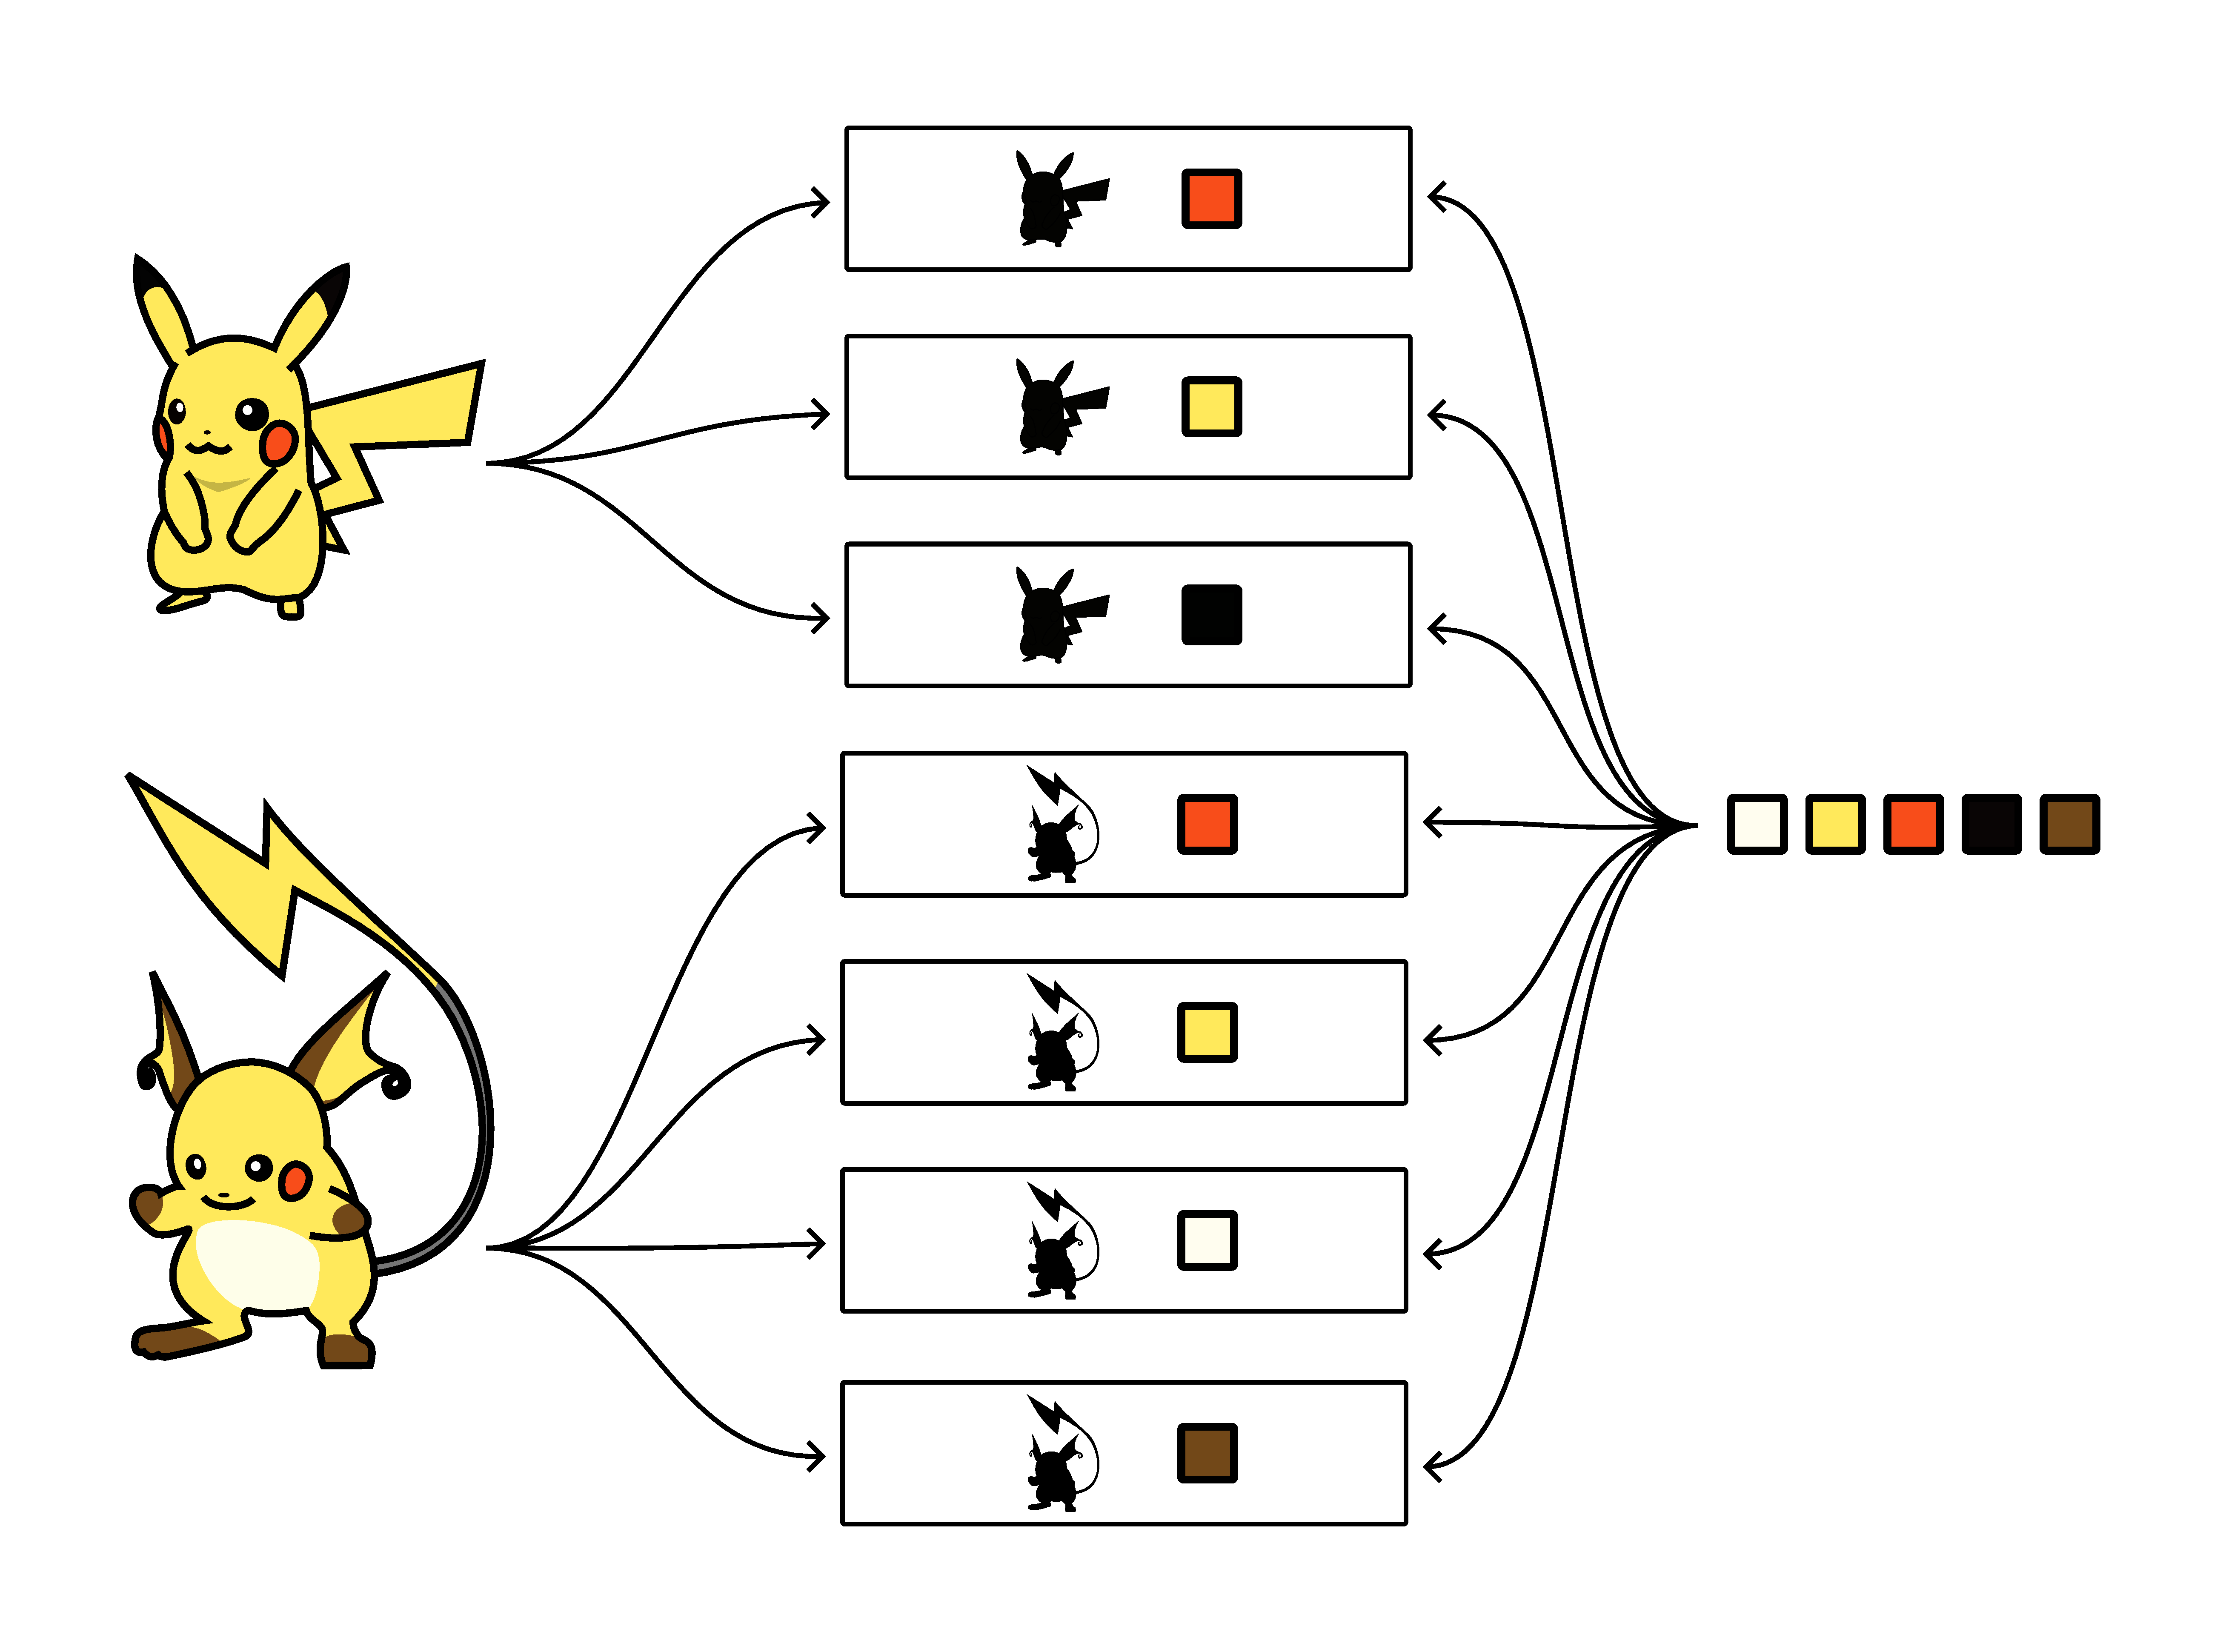
\includegraphics[width=\textwidth]{Images/Fig4}
  \caption{\textit{\textbf{The colors of Pikachu and Raichu}:
By adding statements for the non-exclusive character for the color of Pikachu and Raichu, the user can pick and/or exclude freely from a list of colors in the identification key.
}}
 \label{fig4}
\end{figure}

\section*{
Discussion
}
The examples provided here illustrate the versatility of a format as Clavis. Several of its features are, to our knowledge, not supported by any other format, nor is the totality of its features.

A crucial aspect in identifying any taxon is the geographic origin of the target specimen. Primarily, it dictates which taxa are candidates for its true identity, and thus which key can be used and which taxa within the key are to be considered. Secondarily, it dictates the possible traits of the taxa, insofar as these vary geographically. By referring to external services for geographical information, keys can be made to directly benefit from Species Distribution Models hosted elsewhere, ever improving as more data and improved methodology become available.

\begin{figure}[!h]
  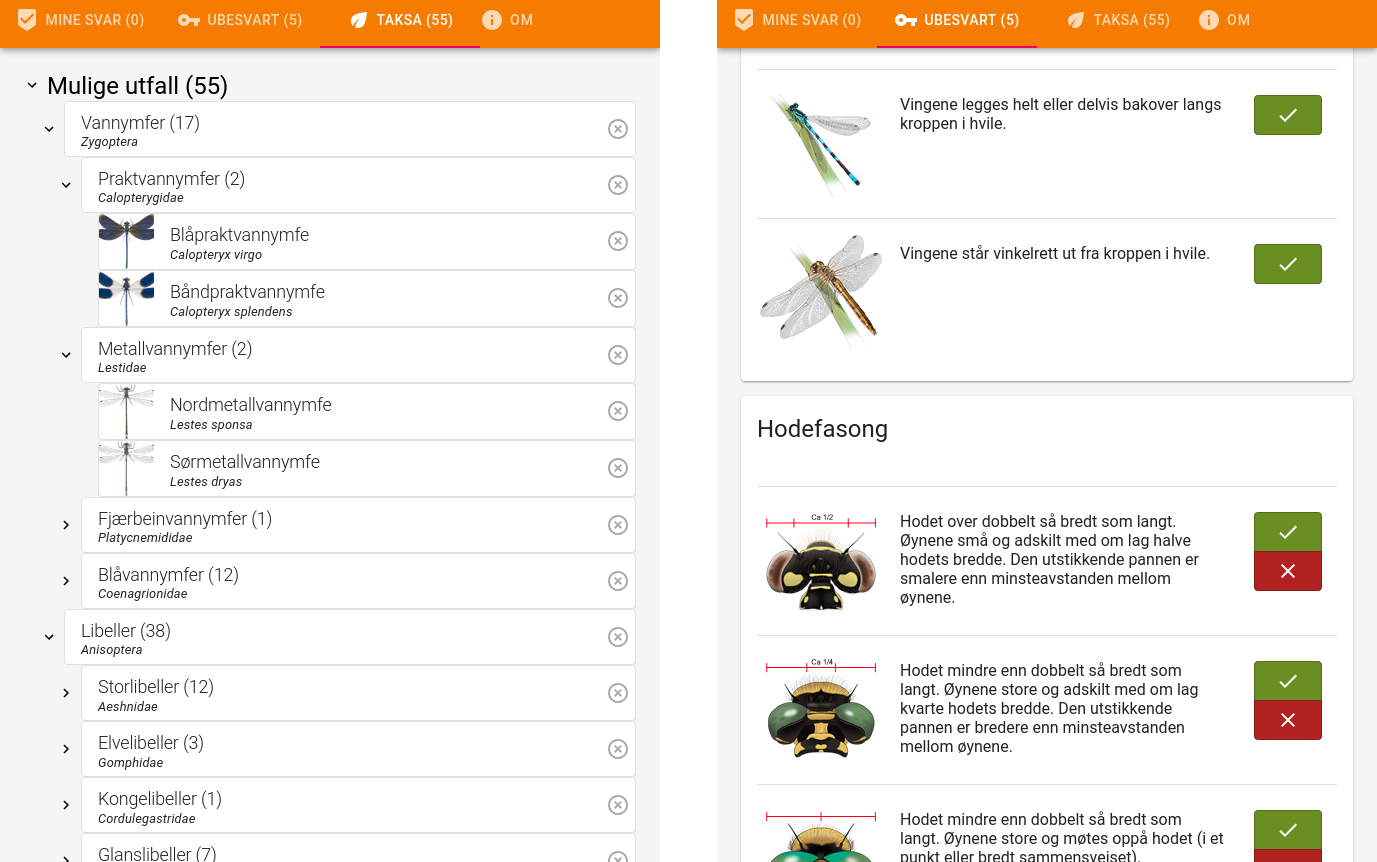
\includegraphics[width=\textwidth]{Images/Fig5}
  \caption{{\bf An example implementation of a Clavis key graphical user interface.}
A hierarchical list of taxa (left) is reduced by providing input on characters (right). Only characters relevant for all remaining taxa are shown.
}
  \label{fig5}
\end{figure}

It is important to realize that keys are designed to function as a whole, and that its content needs to be regarded in context of the whole. While it may in some cases be possible to extract traits from a key for use in a different context, taxonomic knowledge is required to assess the relevance of such traits outside of the key's context. Characteristics defined in the context of distinguishing between taxa within a limited taxonomic and geographical scope can be misleading when put in contexts other than that of the key.

A particularly potent application of the Clavis format will be an implementation in tandem with automated image recognition. Due to the fact that statements are stored as separate entities, there is no fixed path through a key where taxa are evaluated against their characteristics in any particular order. This means that any subset of taxa covered by a key can be distinguished between, without requesting superfluous information from the end user. This allows for a reduction of the probable identifications by a machine learning algorithm as a first step, using a relevant subset of the key to make a final determination. This mechanism potentially reduces the need for much of the user input of a full key, thus reducing the possibility of providing incorrect input that is inherent with each time user input is provided. Conversely, it reduces the reliability solely on machine learning for identification, providing a mechanism of quality controlling the algorithms output, and an opportunity for the end user to learn a great deal more than they would with only a recognition model prediction.

The development of Clavis has been done in close collaboration with taxonomic experts. While this has enabled us to include many diverse features covering needs that have arisen in the past, no such endeavor can expect to produce a final version covering all needs. Further adoption may also bring to light room for different interpretations that will need to be addressed. Our aim is to continue to update the format, releasing new iterations with improvements. Use of previous versions will remain possible, while we aim to maintain backwards compatibility wherever possible. We invite the community to contribute to the development of Clavis, through submitting issues on GitHub, and resolving issues by answering questions or proposing code changes through pull requests. We hope that solutions supporting Clavis, be it key building software or end-user interfaces, both of which we plan to create examples of, will be shared openly as part of a broader ecosystem of use and re-use.

Our aim is for Clavis to be a relevant tool for storing taxonomic knowledge needed for identification in a way that allows for the representation of the complexity and nuances inherent to such knowledge. The open exchange of taxonomic knowledge, unambiguously captured with as much of the auxiliary details needed for its application, is essential for the preservation of invaluable, increasingly elusive knowledge.

We believe that the storage of taxonomic knowledge with the level of detail exemplified here, combined with user interfaces making it accessible, is vital in enabling observers to gather the data needed for apt nature management. Particularly within citizen science, the potential of tools built on an identification key format such as Clavis is considerable. The more accessible this expert knowledge is, the more accurate the identifications made by the user, and keys on generally less well-known taxa can aid in closing the taxonomic gaps in the data corpus. When storing the user input together with a reported observation, this provides important metadata on the identification and its quality. The result of these projected advances in data collection quality feed back into the areas where these data are used, from research and spatial distribution models to the decision making processes related to the biodiversity crisis in a changing world.

\section*{
Data availability and licensing
}

The latest formal definition of Clavis can be found at \url{https://github.com/Artsdatabanken/Clavis}. All files related to this manuscript can be found at \url{https://github.com/WouterKoch/Clavis}.

Fig. \ref{fig5} is based on an Odonata key previously published by the Norwegian Biodiversity Information Centre. In these screenshots, character illustrations are made by Hallvard Elven and licensed under a CC BY 4.0 license, while taxon images are made by Göran Liljeberg and licensed under a CC BY-SA 4.0 license.

Pokémon and its characters are the intellectual property of The Pokémon Company International. The depictions of Pokémon characters in this manuscript are hand drawn fan art by the authors. Both fan art and scientific use constitute fair use in this context. While reuse is governed by the license under which this paper is published, use of these images in contexts that do not constitute fair use may infringe on trademark rights of The Pokémon Company International. As stated in the license under which this manuscript is published, the authors bear no responsibility for any use by others, and recommend consulting with legal experts or The Pokémon Company International prior to reuse to avoid dispute.

\section*{
Supporting information
}

\paragraph*{S1 Appendix.}
\label{S1_Appendix}
{\bf Clavis JSON-schema.} The formal definition of what constitutes a Clavis-compliant key.

\paragraph*{S2 Appendix.}
\label{S2_Appendix}
{\bf Pokémon key example.} A Clavis-compliant key to a number of Pokémon. Serves to illustrate all the different aspects that Clavis supports, rather than to provide a fully functional and complete key.

\paragraph*{S3 Appendix.}
\label{S3_Appendix}
{\bf Titmice key example.} A Clavis-compliant key to Norway's titmice (Paridae). Serves as a real life example of a fully functional and complete key, using only a selection of Clavis' capabilities.

\section*{
Acknowledgements
}
We are grateful to Askild Aaberg Hofsøy Olsen for his feedback on the technical aspects of the Clavis schema. 
\nolinenumbers
\bibliography{Clavis}
\end{document}
